\section{Allgemeine Beschreibung}
\subsection{Aufgabenstellung und Umsetzungsansatz}
Die Aufgabestellung des Semesterprojektes ist es eine Hochregallagersimulation unter zuhilfenahme eines Echtzeitbetriebssystems zu erstellen. Diese soll das gesamte System mit einer statisch gewählten Regaldimension sowohl steuern als auch simulieren.
Das Simulationmodell umfasst ein Regallagersystem mit $5*10$ Regalfächern, ein Ein- und ein Ausgabeslot und einen Turm zum be- und entladen. Dieser Turm ist auf einer Achse montiert auf welcher er sich in X-Richtung bewegen kann, desweiteren kann der Ausleger am Turm in Y-Richtung herauf und herab. An dem Ausleger ist widerum ein Schlitten befestigt welcher in Z-Richtung rein, also zum Hochregal hin, und raus, zu den Ein-/Ausgabe-Slots gefahren werden kann. Die Position dazwischen wird als neutrale Position bezeichnet. Sämtliche Bewegungen des Turms werden von Tastern auf den Schienen ermittelt um daraus die Position des Turmes bestimmen zu können.\\
Auf der X-Achse und auf der Y-Achse befinden sich jeweils 10 Taster und auf der Z-Achse 3.

Um ein Klötzchen vom Eingabe-Slot oder aus einem Regalfach aufzunehmen wird der Schlitten am Ausleger unterhalb des Klötzchens aus der neutralen Position der Z-Achse in den Slot bzw. das Fach gefahren und dann erst angehoben. Umgekehrt wird beim Ablegen eines Klötzchens in den Ausgabe-Slot oder in ein Regalfach das Paket von oben auf den Slot bzw. das Regalfach abgesenkt bevor der Ausleger am Schlitten  in die neutrale Position der Z-Achse zurückgefahren wird.
\begin{figure}[H]
	\centering
  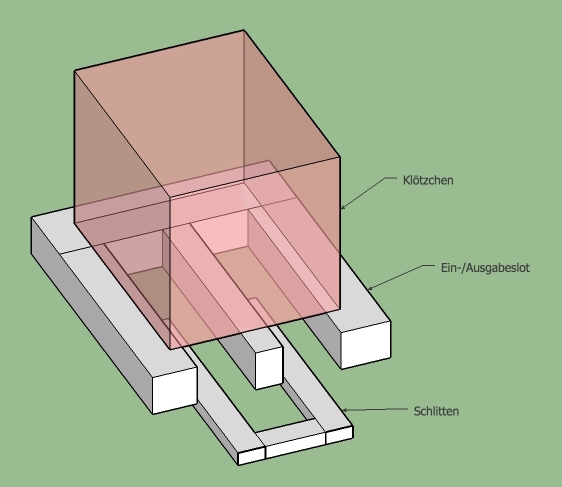
\includegraphics[width=0.45\textwidth]{diagrams/vonunten.jpg}
  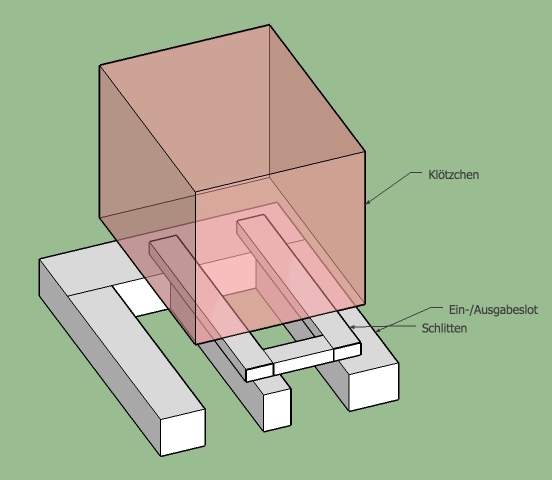
\includegraphics[width=0.45\textwidth]{diagrams/auflegernachoben.jpg}
	\caption{Aufnahme/Ablage an Ein-/Ausgabe-Slot}
	\label{fig2}
\end{figure}

Zur Eingabe- und Ausgabe steht dem Bediener die Konsole zur Verfügung.
\newline\newline
Folgende Befehle werden zur Verfügung gestellt:
\begin{itemize} 
	\item getspace $\rightarrow$ Zeigt aktuelle Belegung des Hochregallagers an
	\item vsetspace[x][y] $\rightarrow$ Definiert einen Platz als schon belegt
	\item clearspace[x][y] $\rightarrow$ Definiert einen Platz als frei
	\item insert[x][y] $\rightarrow$ Holt ein Klötzchen vom Eingabe-Slot und legt es an gewünschter Position im Hochregallager ab
	\item remove[x][y] $\rightarrow$ Holt ein Klötuchen von der gewünschten Position ab und legt es an den Ausgabe-Slot
\end{itemize}

Sollte ein Befehl nicht möglich sein, da zum Beispiel ein Hochregallagerplatz oder der Ausgabe-Slot bereits belegt ist, wird der Anwender durch eine Fehlermeldung in der Konsole darauf aufmerksam gemacht und der Befehl nicht ausgeführt.

Die Visualisierung des Hochregallagers erfolgt ebenfalls in der Konsole, in welcher sowohl das Hochregal und dessen Belegung als auch die Position des Turms und dessen Auslegers, durch ASCI-Zeichen stilisiert dargestellt werden.
Dabei liegt der Ursprung der Koordinaten und somit der Regalplatz (0,0) in der linken unteren Ecke.
Die Darstellung des Ein- und Ausfahren des Auslegers wird unterhalb dargestellt. Dabei stellt die linke Position den zum Ein-/Ausgabe-Slot gefahrenen Arm da, die rechte Position die in das Regal hereingefahrene.
\todo{Bild der Konsole einfügen}

\subsection{Entwicklungsumgebung und Programmierung}
Als Entwicklungs- und Testumgebung wurde Windriver Workbench 3.3 genutz und die Programmiersprache C verwendet.
Es wurden für das Echtzeitbetriebssystem Vxworks Libaries inkludiert.


